\chapter{Implementation} \label{sec:implementation}

Since no existing suitable datasets existed prior to this work, we first create
a dataset for use on this problem. We then create a controlnet-based model for usage on the dataset.

\section{Data Sources}

% \begin{itemize}
%   \item Satellite - JEZ GeoTiff from Mars Trek
%   \item DEM - JEZ GeoTIFF from HiRISE release \url{https://www.uahirise.org/ESP_059352_1985}
%   \item Ground Imagery - PDS data node beta archive explorer \url{https://pds-imaging.jpl.nasa.gov/beta/archive-explorer}
% \end{itemize}

Data was all sourced from publicly available NASA resources.

The Ground imagery was collected from NASA Jet Propulsion Laboratory's Planetary
Data Systems data node, filtered for cylindrically projected mosaic panoramic
images released from the Perseverance rover \cite{PDS_IMG_Node_Mars2020}.

The satellite views were sourced from processed GeoTIFF map data released by
NASA as part of the planning for landing the Perseverance rover in the Jezero
crater region. This data was initially collected from the GeoTIFF released as a
part of the Mars Trek application \cite{MarsTrek_Law2017}, but was later swapped
to use data from the slightly less comprehensive Jezero crater region HiRISE
data release for consistency with the DEM data.

The DEM data was sourced from the HiRISE data release done by the USGS
\cite{USGS_Mars2020_TRN_HiRISE_2020}.

\section{Data Processing Pipeline}

\subsection{Ground Imagery}

% \begin{itemize}
%   \item VICAR Images
%   \item Normalization
%   \item Gamma correction
%   \item Reprojection
%   \item Resizing
% \end{itemize}

The Perseverance ground imagery's native form is in VICAR format, and so imagery
was opened using a patched version rms-vicar, a python-based VICAR file reader
maintained by SETI \cite{hinchliff2025rms‐vicar}. While PNG releases of
converted images are also done, VICAR was chosen as the imagery source since the
specifics of the imagery conversion and if any data is lost is unknown to us.

Since imagery contained absolute intensity instead of sRGB image data, it was
first normalized and then gamma corrected ($\gamma = 2.2$), for usage as
standard 24-bit PNG image data.

The associated PDS label data in the VICAR images was extracted and stored in a
metadata csv file, for later usage in processing the satellite imagery.

Since the mosaic imagery often had different extents and orientations (sometimes
being only a small portion of a much larger image), it needs to be reprojected
to a standard panoramic form for usage in machine learning.

This was done using a Python and OpenCV to build a remap operation to shift the
view and height to approximate a uniform perspective for the imagery. The
details of the reprojection formulae is included in
Appendix~\ref{sec:awful-reprojection-math}.

\begin{figure}

\begin{tikzpicture}[
  io/.style={
    draw=black
  },
  stage/.style={
    draw=black
  },
  descr/.style={
    fill=white,
    inner sep=2.5pt
  }
]
  \node [io] (raw) {
    \includegraphics[width=0.30\linewidth]{N_LRGB_0124_RZS_0041678_CYL_L_AUTOGENJ03_raw.jpg}
  };

  \node [stage, right=of raw] (reproj) {
    \begin{minipage}{0.2\linewidth} % adjust width for your layout
        \centering
        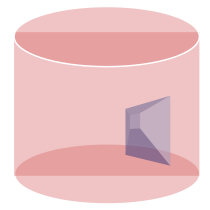
\includegraphics[width=\linewidth]{reproj-icon.jpg} \\
        Reprojection
    \end{minipage}
  };

  \node [io, right=of reproj] (projed) {
    \includegraphics[width=0.30\linewidth]{N_LRGB_0124_RZS_0041678_CYL_L_AUTOGENJ03_proj.jpg}
  };

  \draw[-stealth] (raw.east) |- (reproj.west);
  \draw[-stealth] (reproj.east) |- (projed.west);
\end{tikzpicture}


\caption{Ground processing pipeline reprojection example, showing a ground image reprojected into a standardized cylinder.}
\label{fig:ground-pipeline}

\end{figure}

Lastly, the images were resized to be 1024x512, an arbitrary size comparable to
other works done in the field.

\subsection{Satellite Imagery}

% \begin{itemize}
%   \item HiRISE GeoTIFF
%   \item SPICE localization lookup
%   \item GDAL tile cropping
%   \item Blender ground view reprojection
% \end{itemize}

The ground imagery does not contain localization information trivially
convertible to latitude and longitude. Position information is given in a
Mars-fixed Cartesian frame relative to a recursively defined "site frame", where
the first site frame is defined relative to the rover landing location and the
second site frame is defined relative to the first, etc.

We sidestep this complexity by instead locating the rover based on the time the
image was assembled into a mosaic panorama and looking up it's position in
public releases of rover localizations. In our work, we used publicly available
SPICE data to do this \cite{mars2020_spice_kernels_2025}. We may have been able
to use the simpler PLACES database, but is has a lower temporal resolution of
only one position per day and no inbuilt interpolation. Using python and
SpiceyPy, we looked up the latitude and longitude of the Perseverance rover at a
given time when a mosaic image was assembled \cite{SpiceyPy_Annex2020}. Since
most mosaics are assembled while the rover is still at the location of the
mosaic images, this provides a good heuristic for the rover's approximate
location.

For each located image, a 0.005\textdegree{} diameter tile of satellite image
and DEM data was extracted from the full data release using Python and GDAL
\cite{USGS_Mars2020_TRN_HiRISE_2020, GDAL_2025}. This comes out to a 1124 by
1186 tile of the satellite image data at 25 cm/pixel, and a 296 by 296 tile of
the DEM image data at 1 m/pixel. This makes the absolute extent of each tile
just under 300 m diameter.

\section{Ground View Reprojection}

Models trained using only the overhead satellite view as the prior were found to
be able to create realistic looking results, but often struggled to reconstruct
terrain accurately. This is reflected in our quantitative evaluation of these
models in \cref{sec:results} as well as the outputs in
appendix~\ref{sec:full-test-results}.

We believe this is likely because the U-Net architecture used in the diffusion
backbone of Stable Diffusion 2.1 struggles to encode the quite complex
non-linear perspective shifts in the data, and as such struggles to converge
into a useful result. This is consistent with the work of
\citeauthor{li2024crossviewdiff}, where they chose to use a ground view sky mask
to guide the diffusion process \cite{li2024crossviewdiff}. We do not have access
to sky mask data, and don't want to use it as a prior, so chose to instead use a
conceptually similar approach of reprojecting the satellite view tiles into the
ground view space to make the perspective shift minimal.

This was done using Blender, an open source 3D graphics suite that includes a
robust scripting API \cite{blender2025}. The satellite view was projected onto a
plane of size 2.0 units. The plane was then subdivided in accordance with the
resolution of the ground DEM texture, and then the DEM texture was applied as a
displacement modifier to the plane. The plane was then offset by the scaled
height of the displacement height under the camera (the center of the texture),
such that the displaced plane would remain fixed near the scene origin. From
empirical testing, we found that a displacement strength of 0.1 and a camera
height of 0.25 units produced results reasonably consistent with the ground view
imagery.

The full data processing pipeline is visualized in \cref{fig:data-pipeline}.

\begin{figure}

\begin{tikzpicture}[
  io/.style={
    draw=black
  },
  stage/.style={
    draw=black,
    minimum height=0.5\linewidth,
    minimum width=0.2\linewidth
  },
  descr/.style={
    fill=white,
    inner sep=2.5pt
  }
]

  \node [stage] (gdal) {
    \begin{minipage}{1.5cm} % adjust width for your layout
        \centering
        \rotatebox{270}{GDAL Tile Extraction}\\[2pt]
        \includegraphics[width=\linewidth]{gdalicon.png}
    \end{minipage}
  };

  \node [io, above left=-3.4cm and 1cm of gdal] (rgbfull) {
    \includegraphics[height=0.18\linewidth]{JEZ_hirise_soc_007_orthoMosaic_25cm_Ortho_blend120_thumb.png}
  };

  \node [io, below=of rgbfull] (dtmfull) {
    \includegraphics[height=0.18\linewidth]{JEZ_hirise_soc_006_DTM_MOLAtopography_DeltaGeoid_1m_Eqc_latTs0_lon0_blend40_thumb.png}
  };

  \node [io, above right=-3.4cm and 1cm of gdal] (rgbtile) {
    \includegraphics[height=0.18\linewidth]{N_LRGB_1252_RZS_0590000_CYL_L_AUTOGENJ03_sat.png}
  };

  \node [io, below=of rgbtile] (dtmtile) {
    \includegraphics[height=0.18\linewidth]{N_LRGB_1252_RZS_0590000_CYL_L_AUTOGENJ03_dem.png}
  };

  \node [io, above=of gdal] (ground) {
    \includegraphics[height=0.18\linewidth]{N_LRGB_1252_RZS_0590000_CYL_L_AUTOGENJ03.png}
  };

  \node [stage, below right=-3.4cm and 1cm of rgbtile] (blender) {
    \begin{minipage}{1.5cm} % adjust width for your layout
        \centering
        \rotatebox{270}{Blender Reprojection}\\[2pt]
        \includegraphics[width=\linewidth]{blender_icon_128x128.png}
    \end{minipage}
  };

  \node [io, below left=1cm and -3cm of blender] (vis) {
    \includegraphics[height=0.18\linewidth]{N_LRGB_1252_RZS_0590000_CYL_L_AUTOGENJ03_vis.png}
  };

  \draw[-stealth] (ground.south) to node[descr] {Rover Mosaic Creation Time} (gdal.north);
  \draw[-stealth] (rgbfull.east) |- ([yshift=2cm]gdal.west);
  \draw[-stealth] (dtmfull.east) |- ([yshift=-2.25cm]gdal.west);
  \draw[-stealth] ([yshift=2cm]gdal.east) |- (rgbtile.west);
  \draw[-stealth] ([yshift=-2.25cm]gdal.east) |- (dtmtile.west);
  \draw[-stealth] (rgbtile.east) |- ([yshift=2cm]blender.west);
  \draw[-stealth] (dtmtile.east) |- ([yshift=-2.25cm]blender.west);
  \draw[-stealth] (blender.south) -- ++(0,-0.5) -| (vis.north);

\end{tikzpicture}


\caption{Satellite imagery processing pipeline, where the time is taken from
ground truth imagery to locate the rover's position, from which tiles are sliced
from the full satellite imagery and DEM data. This is then fed into a
blender-based reprojection script for the production of the final imagery.}
\label{fig:data-pipeline}

\end{figure}

\subsection{HuggingFace Dataset Conversion}

For compatibility with the HuggingFace datasets library, a script was created to
allow for a custom loading of the dataset. This was first written using the
HuggingFace datasets api and python library for a custom scripted dataset, but
with the depreciation of custom scripts (for security reasons) in HuggingFace
datasets v4.0.0, the script was updated to use the imagefolder dataset loader.

This provides additional benefits in that the train and test partitions are
simple directories, allowing them to be more easily used for other problems such
as for calculating results.

\subsection{Train Test Split}

The dataset was split into two partitions, a train split and the holdout test split using a simple random sampling, with 80\% train split and 20\% test split.

\section{ControlNet Model} \label{sec:controlnet-model}

A controlnet model based on Stable Diffusion 2.1 was trained on the projected
ground view imagery. This was trained using a script originally created to fine
tune stable diffusion 2.1 models, and was subsequently modified to automatically
split and optionally appropriately mask the train images. The model was trained
on the dataset with a learning rate of $lr = 10^{-5}$ for 1000 epochs on 2x
NVIDIA V100 GPU. To conserve memory and allow for faster train, 16-bit floats
were used for the model.

% \subsection{Image Splitting} \label{sec:image-split}

% The Stable Diffusion 2.1 foundation model our work builds off of was only designed initially to produce square images. This presents an issue for our 1024x512 images present in our work. We address this with the rather inelegant solution of splitting the images horizontally into two 512x512 images, on which the model is trained independently.

\subsection{Loss Function Ground Truth Masking} \label{sec:loss-masking}

A factor that adds additional complexity is that panoramic mosaics that serve as
ground truth imagery can have missing data, and in fact do in almost all cases.
For instance, in \cref{fig:missing-data}, the blacked out regions indicate
a lack of data, not true colors of the image. This is obvious to our eyes, but
less so to a machine learning model, leading it to reproduce these artifacts in
its output. This is undesirable, and so we compensate for it by masking the
predicted image such that the model loss is only computed between the section of
imagery that is truly present in the imagery. This is done by thresholding for
non-black pixels to create a ground image mask. This mask is the applied to the
predicted imagery, and the loss is then subsequently calculated between the
imagery as per normal, as shown in \cref{fig:gt-masking-ex}.

\begin{figure}
\includegraphics[width=\linewidth]{N_LRGB_1252_RZS_0590000_CYL_L_AUTOGENJ03.png}

\caption{Example ground imagery panorama mosaic after reprojection. Blacked out regions indicate areas where the panorama is missing data.}
\label{fig:missing-data}
\end{figure}

\begin{figure}

\includegraphics[width=\linewidth]{ground-mask-ex.jpg}

\caption{Example pipeline for ground truth masking the loss, with MSE loss as an example.}
\label{fig:gt-masking-ex}

\end{figure}

\subsection{Joint Ground \& Projected View Masking} \label{sec:mut-masking}

Additional experiments were conducted with masking loss the function on the
intersection between the data present in both the conditioning image and the
true ground imagery. The theoretical basis being that the region of non-black
pixels in both the projected ground view and the true ground view is the only
region where there is an actual overlap in information between the ground imagery
and the satellite patch. Of course, this assumes that the registration of both
images is perfect, which is not the case, however we decided to test this to see
if it could still improve results for the intersection between the views even
given that caveat.

This was done by taking the bitwise and of a mask of both the ground and prior
imagery, then applying that to the predicted imagery and the ground imagery for
loss calculation, as shown in \cref{fig:mi-masking-ex}.

\begin{figure}

\includegraphics[width=\linewidth]{full-mask-ex.jpg}
\caption{Example pipeline for joint masking the loss on only the data present in
both the ground and conditioning imagery, with MSE loss as an example.}
\label{fig:mi-masking-ex}

\end{figure}
